\documentclass{ximera}

%\addPrintStyle{..}

\begin{document}
	\author{Bart Lambregs}
	\xmtitle{De horizontale worp}{}
    \xmsource\xmuitleg


Wanneer een object horizontaal met een bepaalde beginsnelheid wordt gekatapulteerd, noemen we die beweging een horizontale worp. 

Wij beschouwen de worp in het luchtledige.
\begin{image}[0.6\textwidth]

	% TODO: NOG DE STARTPOSITIE MET V_0 INVOEGEN.

	\begin{tikzpicture}[xscale=0.5, yscale=0.5]
		% \draw[thick,->] (0,0) -- (10,0) node[right] {$x$};
		% \draw[thick,->] (0,0) -- (0,10) node[above] {$y$};
	
		% \foreach \x in {1,...,10}
		%     \draw (\x,0) -- (\x,-0.2) node[below] {\x};
		% \foreach \y in {1,...,10}
		%     \draw (0,\y) -- (-0.2,\y) node[left] {\y};
		
		% Projectile parameters
		\def\v{15}          % Initial speed
		\def\theta{0}     % Launch angle in degrees
		\def\g{50}       % Gravity
		\def\vel{1}      % length of velocity vector
		\def\hoogte{3}  
		\def\imgsize{0.5cm}   
	
		% Trajectory
		\draw[thick, orange, domain=0:10, samples=50, smooth, dotted] 
			plot (\x, {tan(\theta)*\x - ( \g / (2 * \v * \v * cos(\theta)^2) ) * (\x)^2 + \hoogte});
		


		% Ball positions + velocity vectors in a single loop
		\foreach \x [count=\i] in {0,2,4,...,8} {

	
			% y-coordinate
			\pgfmathsetmacro{\y}{tan(\theta)*\x - ( \g / (2 * \v * \v * cos(\theta)^2) ) * (\x)^2 + \hoogte}
			% derivative (slope)
			\pgfmathsetmacro{\slope}{tan(\theta) - (\g / (\v*\v*cos(\theta)^2))*\x}
	
			\pgfmathsetmacro{\arrowHeadsize}{0.3*\vel} % you can replace with a more complex formula
	
	
			% Ball position (red dot or image)
			% \fill[red] (\x,\y) circle (1.5pt);
			\node at (\x,\y) {
\includegraphics[width=\imgsize]{basketbal}}; % optional
			
			% Velocity vector tangent to trajectory
			% \draw[->, blue, very thick, -latex] (\x,\y) -- ++({\vel/sqrt(1+\slope*\slope)}, {\vel*\slope/sqrt(1+\slope*\slope)});
			\draw[->, blue, very thick, -latex] (\x,\y) -- ++(\vel, {\vel*\slope}) node[blue, pos=0.8, right]{\(\vec{v}_{\tiny \i}\)};
			\fill[blue] (\x,\y) circle (2pt);

			\ifnum \x=0 
			\else 
			% Velocity decomposition
			% x-component
			\draw[->, red, thick, -latex] 
			(\x,\y) -- ++(\vel,0) node[above]{\(\vec{v}_x\)};

			% y-component

			\draw[->, purple, thick, -latex] 
			(\x,\y) -- ++(0,{\vel*\slope}) node[below]{\(\vec{v}_{\i, y}\)};
			\fi

			
			% \draw[->, xmgreen, very thick, -latex] (\x,{\y-0.2}) -- ++(0, -1) node[xmgreen, midway, left]{\(a\)};
			% \fill[xmgreen] (\x,{\y-0.2}) circle (2pt);
			
			% \ifnum \x=9
			% \node[xscale=-1, opacity=1] at ({\x+0.2},\y) {
\includegraphics[width=1cm]{basketring}}; 
			% \fi
	
			}
		\end{tikzpicture}
	% 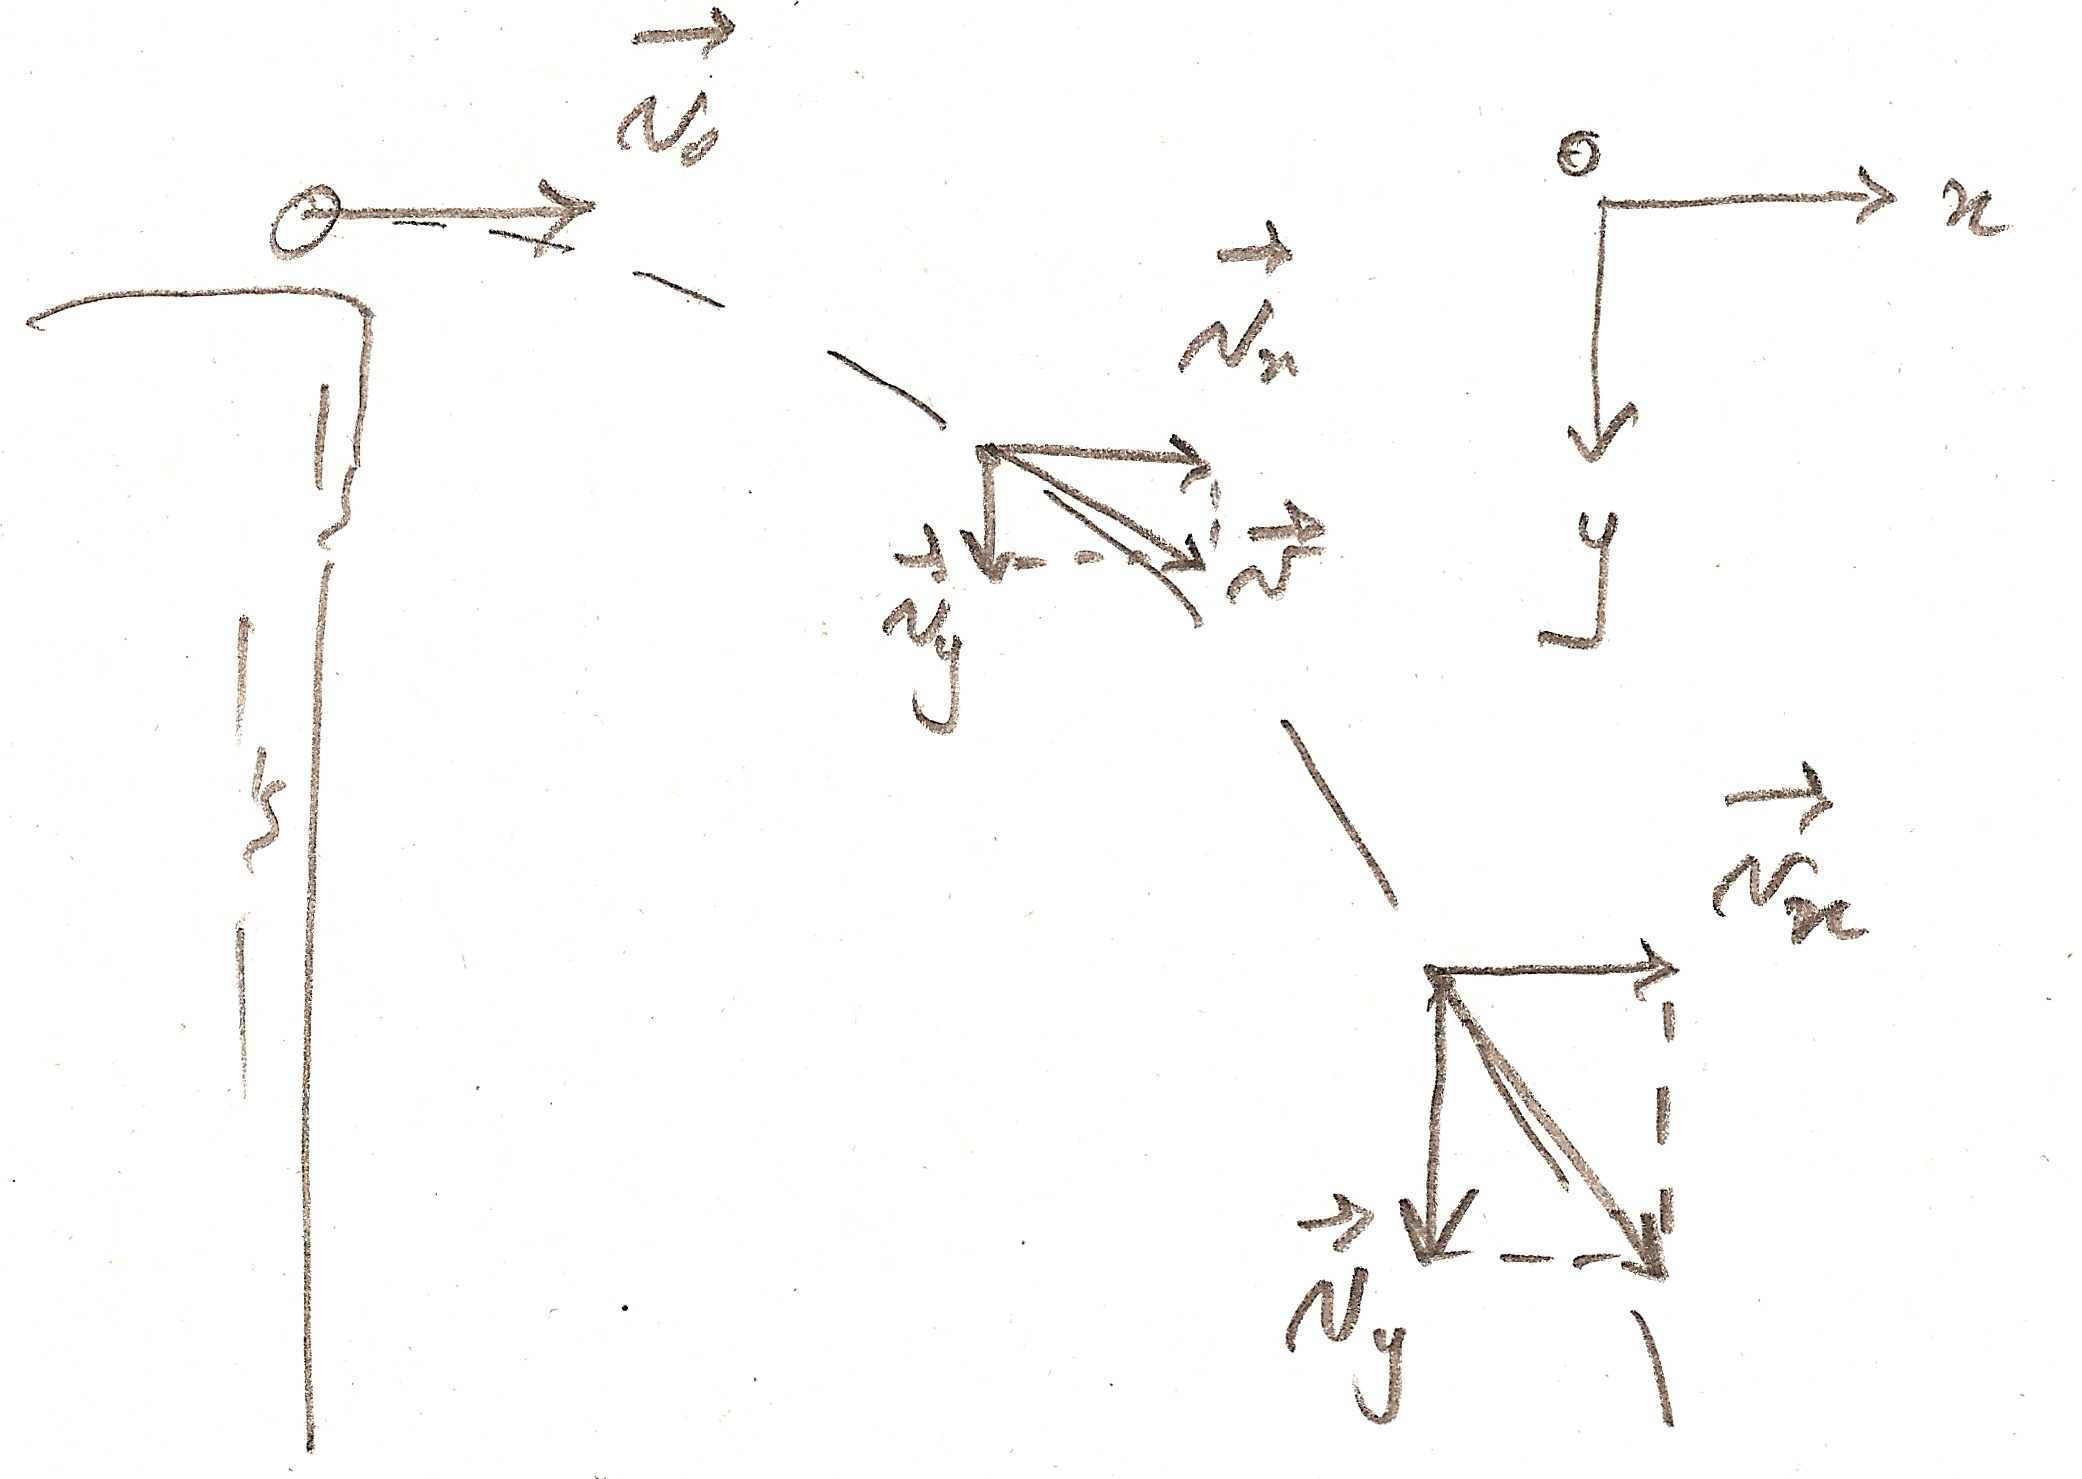
\includegraphics[width=0.6\textwidth]{horizontaleworp_tekening}
\end{image}
\captionof{figure}{De snelheid in horizontale richting verandert niet, die in de verticale richting neemt lineair toe in de tijd}

In de beschrijving kunnen we de $x$-as horizontaal en de $y$-as verticaal naar beneden nemen. Omdat er volgens de $x$-as geen versnelling is het lichaam volgens de $y$-as valt met de valversnelling $g$, kunnen we de formules voor een ERB en een EVRB op de afzonderlijke assen toepassen en zo de volledige beweging beschrijven.
\begin{equation*}
	\left\{
	\begin{array}{l}
	a_x=0\\
	a_y=g
	\end{array}
	\right.
	\Rightarrow
	\left\{
	\begin{array}{l}
	v_x=v_0\\
	v_y=gt
	\end{array}
	\right.
	\Rightarrow
	\left\{
	\begin{array}{l}
	x=v_0t\\
	y=\frac{1}{2}gt^2
	\end{array}
	\right.
\end{equation*}


De baanvergelijking vinden we zoals eerder vermeld, door $t$ in functie van $x$ te schrijven $x=v_0t\Leftrightarrow t=\frac{x}{v_0}$ en dit in $y(t)$ te substitueren:
\begin{eqnarray*}
	y=\frac{1}{2}gt^2=\frac{1}{2}g\left(\frac{x}{v_0}\right)^2=\frac{g}{2v_0^2}x^2
\end{eqnarray*}
De baan is dus (een stuk van) een parabool.

\begin{example}
	Een vliegtuig vliegt met een snelheid van \SI{450}{km/h} op een hoogte van \SI{920}{m}.
	\begin{question} Hoever voor het doel moeten de voedselpakketten gelost worden om op het doel terecht te komen? 
		\begin{oplossing}  
			De afstand waarover de voedselpakketten in horizontale richting zijn vooruit gegaan, kunnen we vinden met de baanvergelijking. We weten namelijk hoever de pakketten naar beneden zijn gevallen en wat hun beginsnelheid is:
			\begin{eqnarray*}
				y&=&\frac{g}{2v_0^2}x^2\\
				&\Downarrow&\\
				x&=&v_0\sqrt{\frac{2y}{g}}=\SI{1712}{m}
			\end{eqnarray*}
		
		\end{oplossing} 
	\end{question}

	\begin{question} Hoeveel tijd hebben de pakketten nodig om het doel te bereiken?                                
		\begin{oplossing}  
		De valtijd voor de pakketten vinden we o.a. door naar de verticale valbeweging te kijken. Deze gebeurt onafhankelijk van wat er in de horizontale richting gebeurt, zodat:

			\begin{eqnarray*}
				y&=&\frac{1}{2}gt^2\\
				&\Downarrow&\\
				t&=&\sqrt{\frac{2y}{g}}=\SI{13,7}{s}
			\end{eqnarray*}
		\end{oplossing} 
	\end{question}




\end{example}
	
\end{document}
